\section{BACKGROUND}
A security framework provides checklist to ensure the integrity of the supply chain.
Artifacts that fulfill SLSA requirements endorsed a traceable source of the software provided
by trusted providers. SLSA provides trustworthiness of the artifacts to the developers, downstream users~\cite{slsa2023}. 

\subsection{What is Software Supply Chain?}
The software supply chain encompasses a complex network of multiple components, including both first-party and third-party libraries, 
as well as various processes integral to the development, build, testing, and publication of a software artifact. 
It serves as the backbone for delivering software products to end-users~\cite{DoDDefCI/CD2023}.

\subsection{Provenance}
SLSA provenance clearly provides the transparent information about the artifacts or the packages.
Information such as, who builds this artifact and how the artifact was built from the source.
The information will be verified by the package registry or even the customers. The provenance
is an attestation in SLSA.

\subsection{SLSA Provenance versus SBOM (Software Bill of Materials)}
Provenance and SBOM are somehow similar, so they are easily confused. Provenance is used to 
assess the trustworthiness and security of the processes used to build and deliver the software artifacts~\ref{provenance}.
By contrast, SBOM focus on listing software components and their versions \ref{SBOM}.

Most software is distributed with pre-compiled package, so inspecting the source code is somehow impossible.
SBOM provides a mapping between binary code and the materials of a software. For example, the version of the 
software will be documented in SBOM. However, the developers cannot trust the pre-compiled artifact is actually 
derived from the authentic source code. Usually, the current trend will tend to build the reproducible artifact which
means the binary code is able to be rebuilt from the source code if using the given hardware. 
Then, the developers can verify the integration through comparing the hash between pre-compiled package and rebuilt artifact~\cite{ferraiuolo2022policy}.

\begin{lstlisting}[language=, caption=SLSA Provenance, label=provenance]
[Software Build Provenance]
Build Date: 2023-09-01
Build Environment: Secure, Isolated Environment
Signing Authority: Trusted Certificate Authority (CA)
Signature Verification: Passed
[Supply Chain Processes]
Code Review: Multi-stage code review by security experts
Dependency Scanning: Automated scanning for known vulnerabilities
Build Automation: Continuous Integration/Continuous Deployment (CI/CD) pipeline
Deployment: Automated deployment to secure servers
[Organizations Involved]
Development Team: Responsible for code development
Security Team: Responsible for security reviews and scanning
Operations Team: Responsible for deployment
\end{lstlisting}

\begin{lstlisting}[language=, caption=SBOM, label=SBOM]
[MyApp (v1.0)]
Frontend Framework (v2.3)
Database Connector (v1.1)
Authentication Library (v3.0)
Logging Utility (v1.2)
\end{lstlisting}

\subsection{Build Model}
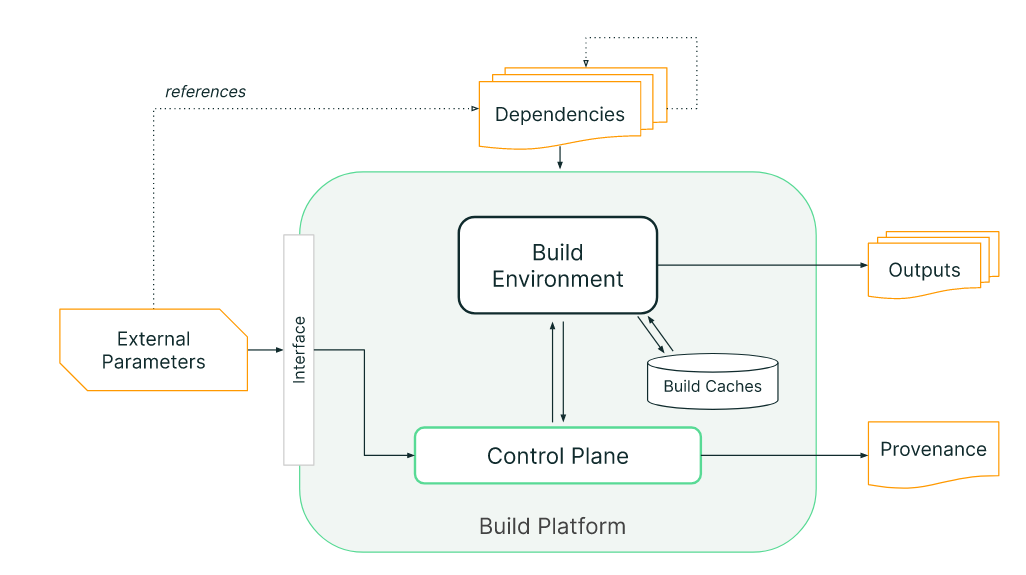
\includegraphics[width=0.7\textwidth]{./screenshot/build_model.png}
\begin{enumerate}
  \item The tenant (developers) provide specific external parameters, like the version of the application 
  and the reference to the dependency.
  \item The control plane receives the external parameters, then fetch the necessary build scripts, configuration,  
  and dependencies based on the external parameters.
  \item The control system sets up the isolated environment for the build.
  \item Finally, the model outputs the artifacts. If the build platform follows SLSA build level 2+, then
  the provenance will also be generated from the control systems.
\end{enumerate}
\subsection{SLSA Security Level}
Currently, SLSA have defined 4 levels (LV.0 - LV.3), which will be 
briefly described in Table~\ref{tab:slsa-levels}, and working on level 4.
\begin{table}[ht]
  \centering
  \caption{SLSA Security Levels}
  \label{tab:slsa-levels}
  \begin{tabular}{|c|c|p{6cm}|}
  \hline
  \textbf{Level} & \textbf{Requirements} & \textbf{Focus} \\
  \hline
  Build L0 & None & No security practices are in place. \\
  \hline
  Build L1 & With provenance & Basic security practices are followed, such as code review and basic dependency scanning. \\
  \hline
  Build L2 & Signed provenance, generated by a hosted build platform & More comprehensive security practices are implemented, including in-depth code review, vulnerability scanning, and build verification. \\
  \hline
  Build L3 & Hardened build platform & The highest level of security is maintained, with strict adherence to security practices, automated testing, and supply chain integrity checks. \\
  \hline
  \end{tabular}
\end{table}

\subsection{Policy Engines}
Policy is a logic code, which will decide whether the action can be operated. There could be
nested policies within on policy. For example, the consumer want to check if they are allowed
to access the cloud and download the data from the cloud. They will if their provided password
valid and whether the source IP is not within the banned IP list. Then, the policy to check whether
the password is valid is based on the correct password format and the password is stored in database.

Policy Engine is able to adopt the results generated from other tools, like the checker in the framework of 
our research or the malicious code injection scanner. The Trusted Wrappers provide and interface to 
convert the results from the original format into the logic. If the policy is verified, it will become 
a fact and store in the Transparency log. Everyone can directly monitor the facts store within the transparency 
log, which prevent the logic from being compromised. The transparency log is untrusted to the consumers,
which means the consumers will not trust the maintainers of the log~\cite{ferraiuolo2022policy}.

Our framework implements the policy engines combined with the result from the check in order to provide a clear 
view and easy way to understand the security requirement of the consumers.


